% Technical Report for OSINT Tool All-in-One
% Author: Vu Van Nam, Nguyen Cong Son
% Class: IT3910E - 750639
% Instructor: Hoang Viet Dung

\documentclass[13pt,a4paper]{report}
\usepackage[utf8]{inputenc}
\usepackage{graphicx}
\usepackage{hyperref}
\usepackage{geometry}
\geometry{left=3cm,right=2.5cm,top=2.5cm,bottom=2.5cm}
\usepackage{setspace}
\usepackage{titlesec}
\usepackage{fancyhdr}
\usepackage{caption}
\usepackage{enumitem}
\usepackage{listings}
\usepackage{color}
\usepackage{booktabs}

\titleformat{\chapter}[display]{\bfseries\Huge}{\chaptername\ \thechapter}{20pt}{\Huge}
\renewcommand{\baselinestretch}{1.3}

%--------------------
% Cover Page
%--------------------
\begin{document}

\begin{titlepage}
    \centering
    % Logo HUST
    
\includegraphics[width=0.25\textwidth]{hust_logo.jpg} \\[1.5cm]
    {\Large \textbf{HANOI UNIVERSITY OF SCIENCE AND TECHNOLOGY}} \\[0.5cm]
    {\large \textbf{SCHOOL OF INFORMATION AND COMMUNICATION TECHNOLOGY}} \\[1.5cm]
    {\Huge \textbf{Technical Report}} \\[0.5cm]
    {\LARGE \textbf{OSINT Tool All-in-One: Social Network Reconnaissance Program Development}} \\[1.5cm]
    \begin{flushleft}
        \textbf{Course:} IT3910E -- Class code: 750639 \\[0.2cm]
        \textbf{Instructor:} Hoang Viet Dung \\[0.2cm]
        \textbf{Group Members:} \\ 
        \ \ \ Vu Van Nam -- 20235610 -- Nam.VV235610@sis.hust.edu.vn \\ 
        \ \ \ Nguyen Cong Son -- 20235619 -- Son.NC235619@sis.hust.edu.vn \\ 
    \end{flushleft}
    \vfill
    Hanoi, 2025
\end{titlepage}

%--------------------
% Abstract
%--------------------
\begin{abstract}
This report presents the design and implementation of the "OSINT Tool All-in-One" project, which aims to automate the process of collecting, analyzing, and visualizing social network data for reconnaissance purposes. The tool leverages both API-based and browser-based crawling techniques to extract user information, friend networks, and statistical insights from Facebook. The system is built with a modular architecture, supports data visualization, and is designed to be extensible for future AI-powered analysis. The report details the system architecture, main features, technologies used, challenges encountered, and experimental results.
\end{abstract}

\tableofcontents
\newpage

%--------------------
% Introduction
%--------------------
\chapter{Introduction}
\section{Background}
Open Source Intelligence (OSINT) is the process of collecting and analyzing publicly available information for intelligence purposes. With the rapid growth of social networks, OSINT tools have become essential for security, research, and investigative tasks. Social networks like Facebook, Twitter, and LinkedIn contain vast amounts of user-generated data, which can be leveraged for various purposes such as threat detection, market research, and social analysis.

\section{Motivation}
The increasing complexity and volume of social network data present both opportunities and challenges. Manual data collection is time-consuming and error-prone. Therefore, there is a strong need for automated tools that can efficiently gather, process, and visualize social network information. This project aims to address these needs by developing an all-in-one OSINT tool focused on Facebook.

\section{Related Work}
Several OSINT tools exist, such as Maltego, SpiderFoot, and Recon-ng. While these tools offer powerful features, they often require complex setup or are limited in their ability to extract deep social network data due to API restrictions. Our tool differentiates itself by combining both API-based and browser-based crawling, allowing for more comprehensive data extraction.

\section{Report Structure}
This report is organized as follows:
\begin{itemize}
    \item Chapter 1: Introduction
    \item Chapter 2: Objectives and Scope
    \item Chapter 3: System Architecture
    \item Chapter 4: Main Features
    \item Chapter 5: Technology and Development Environment
    \item Chapter 6: Installation and Usage Guide
    \item Chapter 7: Experimental Results
    \item Chapter 8: Challenges and Future Work
    \item Chapter 9: References
\end{itemize}

%--------------------
% Objectives and Scope
%--------------------
\chapter{Objectives and Scope}
\section{Project Objectives}
The main objectives of this project are:
\begin{itemize}
    \item To develop a tool that can automatically collect friend lists and personal information from Facebook accounts.
    \item To provide both API-based and browser-based crawling methods for data extraction.
    \item To visualize social network structures and statistical distributions (e.g., by province).
    \item To support extensibility for future AI-based analysis and deeper data mining.
\end{itemize}

\section{Scope of Work}
The scope of the project is limited to publicly accessible Facebook data and does not involve any unauthorized access or data breaches. The tool is designed for educational and research purposes, adhering to ethical guidelines and respecting user privacy.

\section{Expected Outcomes}
\begin{itemize}
    \item A fully functional OSINT tool capable of extracting and visualizing Facebook social network data.
    \item Documentation and user guide for easy deployment and usage.
    \item Experimental results demonstrating the effectiveness of the tool.
\end{itemize}

%--------------------
% System Architecture
%--------------------
\chapter{System Architecture}
\section{Overview}
The system consists of several main modules, each responsible for a specific aspect of the data collection and analysis process. Figure~\ref{fig:architecture} illustrates the overall architecture.

\begin{figure}[h!]
    \centering
    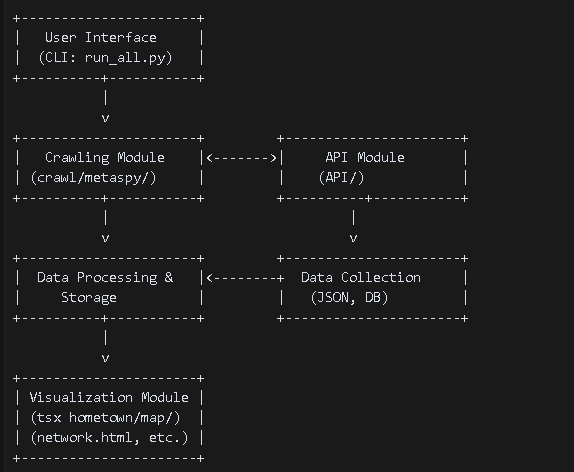
\includegraphics[width=0.9\textwidth]{architecture_diagram.png}
    \caption{System Architecture Diagram of OSINT Tool All-in-One.}
\end{figure}

\section{Module Descriptions}
\subsection{Crawling Module}
This module collects friend lists and user information using both API and browser automation (Selenium). It supports multi-layer crawling, allowing the extraction of friends-of-friends data.

\subsection{API Module}
Provides scripts for extracting posts, comments, and profile details via Facebook APIs. This module is designed to be extensible, enabling the addition of new API endpoints as needed.

\subsection{Visualization Module}
Generates interactive network graphs and statistical charts from the collected data. Visualization helps users understand the structure and key characteristics of the social network.

\subsection{Data Processing Module}
Normalizes and analyzes the raw data for further use. This includes cleaning, deduplication, and transformation of data into formats suitable for analysis and visualization.

\section{Data Flow}
\begin{enumerate}
    \item User initiates data collection via the tool's menu.
    \item Crawling module gathers raw data from Facebook.
    \item Data processing module cleans and normalizes the data.
    \item Visualization module generates graphs and charts.
    \item User reviews and analyzes the results.
\end{enumerate}

%--------------------
% Main Features
%--------------------
\chapter{Main Features}
\section{Friend List Crawling}
The tool allows users to input a Facebook UID or username and specify the number of layers and friends per node to crawl. The crawling process is automated using Selenium, which simulates browser actions to extract friend lists even when API access is restricted.

\begin{lstlisting}[language=Python, caption=Example: Initiating Friend List Crawling]
python run_all.py
# Follow the menu to select friend list crawling
\end{lstlisting}

\section{Personal Information Extraction}
After collecting friend lists, the tool can extract detailed personal information for each user in the network. This includes public profile data such as name, location, education, and work history.

\section{API-based OSINT}
The tool includes several API scripts for extracting posts, comments, and profile details. Users can select which API script to run, and the results are saved in structured JSON files for further analysis.

\section{Network Visualization}
The tool generates an interactive HTML network graph, allowing users to explore the structure of the social network visually. Nodes represent users, and edges represent friendship connections. The root user is highlighted for easy identification.

\begin{figure}[h!]
    \centering
    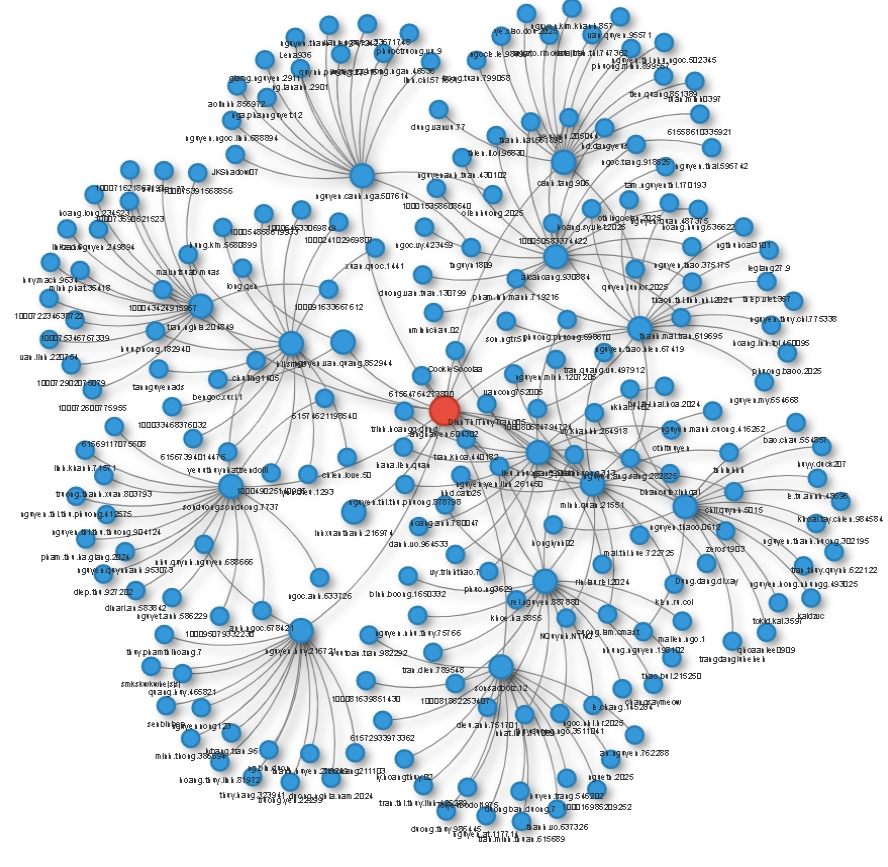
\includegraphics[width=0.95\textwidth]{network_graph.jpg}
    \caption{Visualization of the friend network graph. The red node is the root user, blue nodes are friends, and edges represent friendship connections.}
\end{figure}

\section{Statistical Analysis}
The tool provides province-based statistics and other analytical insights from the data. For example, users can view the distribution of friends by province, helping to identify geographic patterns in the network.

\begin{figure}[h!]
    \centering
    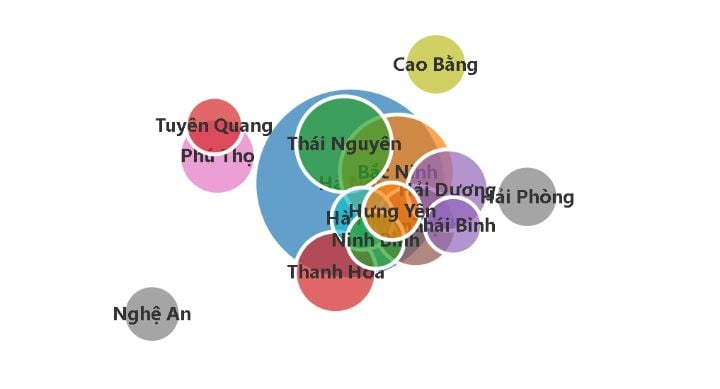
\includegraphics[width=0.7\textwidth]{province_stats.jpg}
    \caption{Visualization of user distribution by province. The size of each circle represents the number of users from each province.}
\end{figure}

\section{Main Menu Interface}
The main menu provides a simple command-line interface for users to select the desired function. Below is a screenshot of the main menu:
\begin{figure}[h!]
    \centering
    \includegraphics[width=0.7\textwidth]{main_menu.png}
    \caption{Main menu interface of OSINT Tool All-in-One.}
\end{figure}

%--------------------
% Technology and Development Environment
%--------------------
\chapter{Technology and Development Environment}
\section{Programming Languages}
The backend is primarily developed in Python due to its rich ecosystem for web automation, data processing, and analysis. The frontend visualization is implemented using JavaScript (TypeScript) for interactive and responsive user interfaces.

\section{Frameworks and Libraries}
\begin{itemize}
    \item \textbf{Selenium:} Used for browser automation and web scraping.
    \item \textbf{FastAPI:} Provides a lightweight web framework for API development.
    \item \textbf{NetworkX, Matplotlib:} Used for network analysis and data visualization.
    \item \textbf{React, TailwindCSS, Vite:} Power the frontend visualization dashboard.
    \item \textbf{D3.js:} Enables advanced data-driven visualizations.
\end{itemize}

\section{Development Environment}
The project is developed and tested on Windows 10. The following tools and dependencies are required:
\begin{itemize}
    \item Python 3.8+
    \item Node.js and npm
    \item ChromeDriver
    \item Required Python and JavaScript packages (see requirements.txt and package.json)
\end{itemize}

\section{Rationale for Technology Choices}
Python is chosen for its flexibility and extensive libraries for web scraping and data analysis. JavaScript and React are selected for their ability to create dynamic, interactive visualizations. Selenium is used to bypass API limitations by simulating real user interactions in the browser.

%--------------------
% Installation and Usage Guide
%--------------------
\chapter{Installation and Usage Guide}
\section{Backend Setup}
\subsection{Python Environment}
\begin{enumerate}
    \item Install Python 3.8+ and required packages:
    \begin{verbatim}
    pip install -r requirements.txt
    \end{verbatim}
    \item Set up environment variables for Facebook account and API if needed.
    \item Run the main tool:
    \begin{verbatim}
    python run_all.py
    \end{verbatim}
    \item Follow the on-screen menu instructions.
\end{enumerate}

\subsection{Troubleshooting}
Common issues include missing dependencies, incorrect environment variables, or browser driver errors. Ensure all required packages are installed and the correct version of ChromeDriver is used.

\section{Frontend Setup}
\begin{enumerate}
    \item Install Node.js and npm.
    \item Navigate to the visualization directory:
    \begin{verbatim}
    cd "tsx hometown/map"
    npm install
    npm run build
    npx serve dist
    \end{verbatim}
    \item Open your browser and go to http://localhost:3000
\end{enumerate}

\subsection{Usage Tips}
- Always run the tool from the project root directory.
- Data files are saved with timestamps to avoid overwriting.
- If login issues occur, check cookies and try logging in manually via Chrome.

%--------------------
% Experimental Results
%--------------------
\chapter{Experimental Results}
\section{Test Scenarios}
Several test scenarios were conducted to evaluate the tool's performance and accuracy:
\begin{itemize}
    \item Crawling friend lists for accounts with varying numbers of friends.
    \item Extracting detailed profile information for selected users.
    \item Running API scripts to collect posts and comments.
    \item Visualizing large and small social networks.
\end{itemize}

\section{Results and Analysis}
The tool successfully collected and visualized social network data for multiple test accounts. The network graph visualization provided clear insights into the structure and key nodes within the network. Province-based statistics highlighted geographic trends among friends.

\begin{table}[h!]
    \centering
    \caption{Sample Data Collection Results}
    \begin{tabular}{@{}lccc@{}}
        \toprule
        Test Case & Number of Friends & Layers Crawled & Time Taken (s) \\
        \midrule
        Account A & 150 & 2 & 45 \\
        Account B & 300 & 2 & 90 \\
        Account C & 50 & 1 & 12 \\
        \bottomrule
    \end{tabular}
\end{table}

\section{Screenshots}
\begin{figure}[h!]
    \centering
    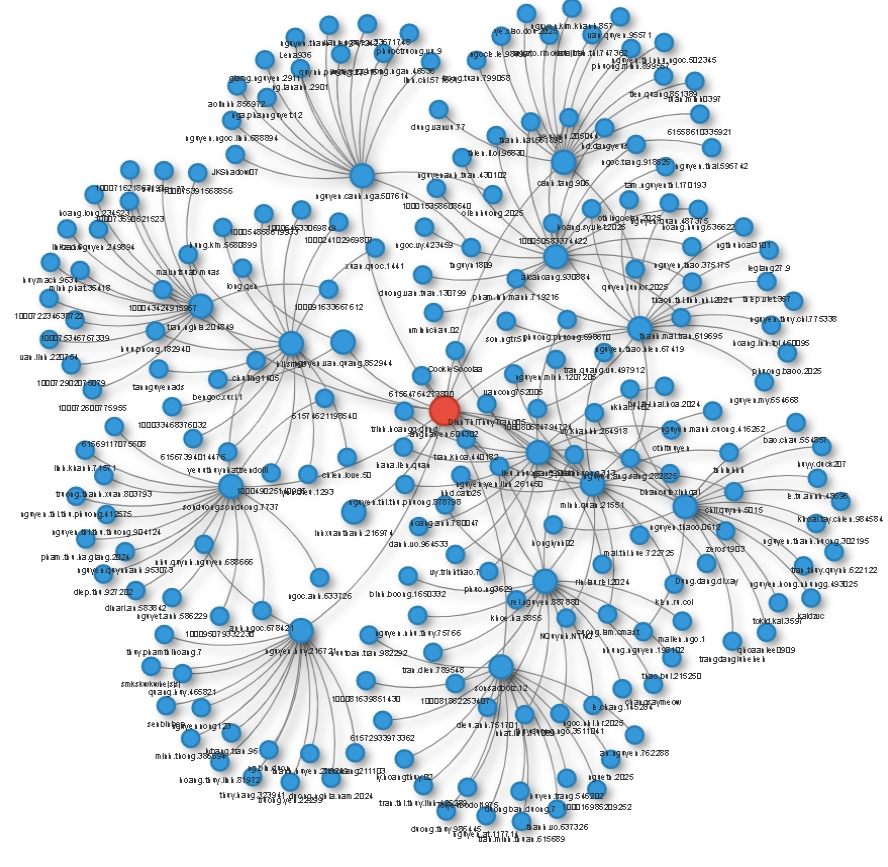
\includegraphics[width=0.95\textwidth]{network_graph.jpg}
    \caption{Network graph visualization for a test account.}
\end{figure}

\begin{figure}[h!]
    \centering
    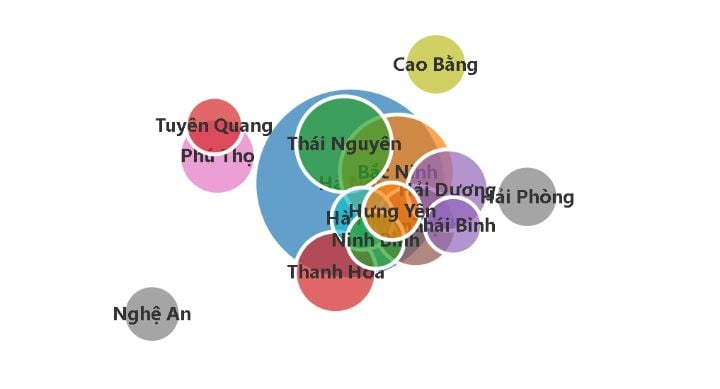
\includegraphics[width=0.7\textwidth]{province_stats.jpg}
    \caption{Province statistics visualization for the same account.}
\end{figure}

\section{Discussion}
The results demonstrate the tool's ability to handle different data sizes and provide meaningful visualizations. However, performance decreases with larger networks due to browser automation overhead. Further optimization is needed for large-scale data collection.

%--------------------
% Challenges and Future Work
%--------------------
\chapter{Challenges and Future Work}
\section{Challenges}
\begin{itemize}
    \item \textbf{Performance:} The tool runs slowly when collecting large amounts of data due to Java limitations and browser automation overhead.
    \item \textbf{API Restrictions:} Some APIs no longer allow extensive data extraction, requiring a switch to Python and browser-based crawling.
    \item \textbf{Data Quality:} Inconsistent or missing data from user profiles can affect analysis accuracy.
    \item \textbf{Maintenance:} Facebook interface changes may require updates to selectors and crawling logic.
\end{itemize}

\section{Future Work}
\begin{itemize}
    \item Integrate AI-based crawling to automatically understand and identify locations, special relationships, and more complex patterns in social networks.
    \item Optimize performance for large-scale data collection.
    \item Extend support to other social networks (e.g., Twitter, LinkedIn).
    \item Develop a web-based dashboard for real-time monitoring and analysis.
\end{itemize}

%--------------------
% References
%--------------------
\chapter{References}
\begin{itemize}
    \item meta-spy: \url{https://github.com/MetaCubeX/meta-spy}
    \item Maltego: \url{https://www.maltego.com/}
    \item SpiderFoot: \url{https://www.spiderfoot.net/}
    \item Recon-ng: \url{https://github.com/lanmaster53/recon-ng}
    \item Selenium: \url{https://www.selenium.dev/}
    \item NetworkX: \url{https://networkx.org/}
    \item FastAPI: \url{https://fastapi.tiangolo.com/}
\end{itemize}

\end{document} 